
Before diving into the architecture of our Crowd-powered Real-time Question Answering (CRQA) system, we will describe the setup of the TREC LiveQA 2016 shared task, which affected some of the system design choices.

A series of TREC LiveQA evaluation campaigns was started in 2015 with the goal to facilitate research in automatic question answering for complex informational needs.
In 2015 and 2016 versions of the task participants of the challenge develop a live question answering system, that needs to respond to user questions, which are sampled from Yahoo! Answers community question answering website live stream.
Each input question consists of the short question title, body and category (Figure~\ref{fig:ya_question}).
A QA system has to provide an answer of 1000 characters or less in under 1 minute time limit.
A reader can refer to \cite{agichtein2015overview} for more details on TREC LiveQA 2015 results and analysis.

\begin{figure*}[h!t]
	\centering
	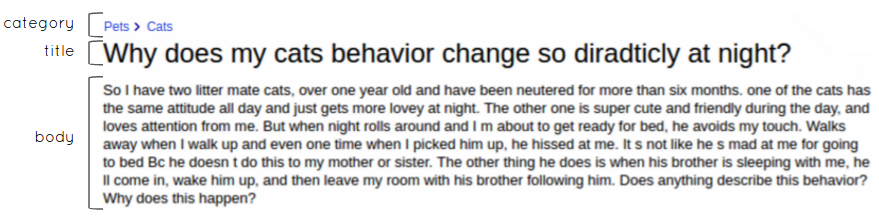
\includegraphics[width=0.8\textwidth]{img/ya_question}
	\caption{Example of the question from Yahoo! Answers community question answering platform}
	\label{fig:ya_question}
\end{figure*}

Our CRQA system represents a hybrid system, that includes an automated question answering and crowdsourcing modules.
The high level architecture is presented in Figure~\ref{fig:system}.

\begin{figure*}[h!t]
	\centering
	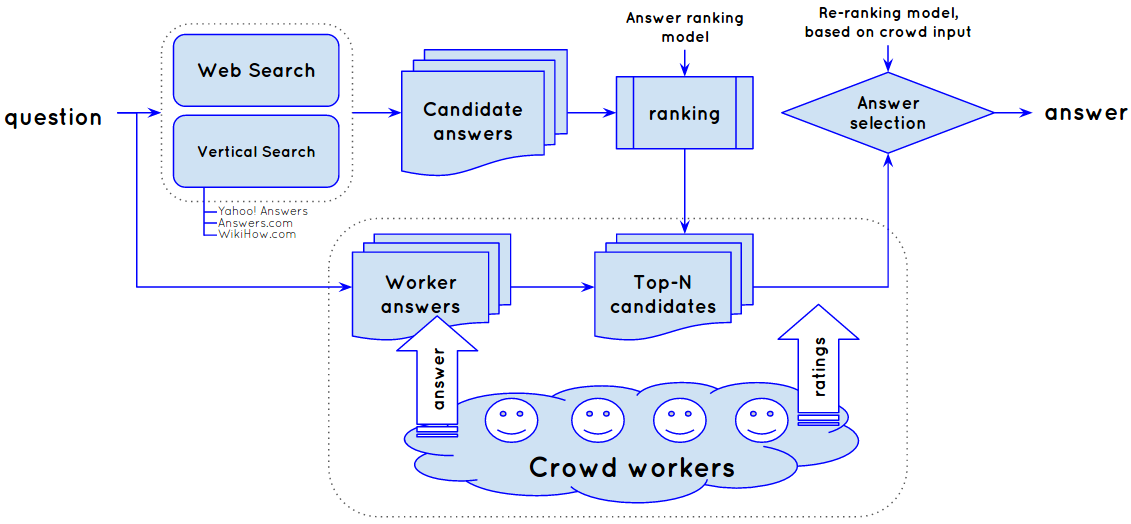
\includegraphics[width=\textwidth]{img/system}
	\caption{The architecture of our Crowd-powered Real-time Question Answering system, that uses crowdsourcing to augment a list of automatically extracted candidate answers and to rate their quality}
	\label{fig:system}
\end{figure*}

The automated part of the CRQA system follows an Information Retrieval (IR) approach to question answering, and generates a set of candidate answer passages from multiple data sources.
After candidates are generated, they are ranked by a trained model, and in the fully automated mode the top candidate could be returned as the answer.
The crowdsourcing module is designed to overcome two of the most common problems of the automated QA approaches: lack of good candidate answers and ranking errors~\cite{moldovan2003performance,savenkov_trecliveqa15}.
More particularly, CRQA asks crowd workers to provide answers to the given questions if they can, and additionally rate the quality of candidate answers, generated by the automated system.
Worker contributions are then used by a trained re-ranking model, that selects the best candidate answers using all the information available.
The next two sections describe the architectures of the automated and crowdsourcing modules of our system.

\subsection{Automated question answering module}
\label{sec:system:auto}

When CRQA receives a question, it generates a set of search queries to retrieve a set of relevant documents and extract candidate answer passages.
Search queries are generated using the following strategies:
\begin{itemize}
\item Question title, which most often captures the gist of the question
\item Two longest question sentences (detected by the presence of the question word at the beginning or question mark at the end of a sentence) from the title and body of the question. In some cases the real user question is hidden inside the body, while the title just provides the overall topic of the question.
\item Concatenation of the question word, verbs and top-5 terms from the question title by Inverse Document Frequency\footnote{IDF of terms are estimated using Google N-gram corpus: https://catalog.ldc.upenn.edu/LDC2006T13}. This strategy targets over-specific questions (\textit{e.g.}, Figure~\ref{fig:ya_question}), which often retrieve few if any search results.
\end{itemize}

To retrieve a set of potentially relevant documents and extract candidate answer passages, CRQA relies on multiple different generic and CQA document collections.
Previous research \cite{shtok2012learning} has shown that many of the user information needs are repeated, and reusing answers to previously posted similar questions is an effective strategy for answering new questions.
Therefore, CRQA uses multiple different CQA data sources, which potentially contain a diverse set of questions.
However, quite often it is hard to find a similar question in an archive, and many of the information needs are unique.
Therefore, we include a web search component, that can retrieve regular web documents, from which our system can extract candidate answers.
More specifically, CRQA queries the web using Bing Web Search API\footnote{https://datamarket.azure.com/dataset/bing/searchweb}, Yahoo! Answers, Answers.com and WikiHow.com using their respective search interfaces.
For each query we retrieve top-10 relevant documents and question-answer pairs from CQA archives.
As candidate answers CRQA extracts answers to the questions retrieved from CQA results and paragraphs of text from the main content of regular web documents, as detected by a method based on \cite{Kohlschutter_2010}.
Quite often, it's hard to estimate the quality of a candidate answers from its text only.
The task becomes much easier if a system has access to additional data, \textit{e.g.} for the candidates generated from the CQA archives, it is useful to know the text of the original question the candidate answers.
For candidates, generated from regular web pages, it's useful to know the topic of the page (\textit{e.g.} from its title), additionally the context of the candidate, such as text that immediately precedes it in the document was shown to provide a useful information for QA.
Therefore, besides the text of a candidate answer, we keep some potentially useful metadata, \textit{e.g.,} for QnA candidates we include text and category of the retrieved question, and web page title and text block preceding the answer passage in the document for web-search based candidates.
For convenience, we will call the title of a retrieved question or web page \textit{``the answer topic''}, and the body of the retrieved question or the preceding text block the \textit{``the answer context''}.

Next, for each candidate answer we compute a set of features, described in Table \ref{table:features}.

\begin{table}[ht]
\centering
\begin{tabular}{| p{8cm} |}
\hline
\textbf{Answer statistics} \\
\hline
--- Length in chars, words and sentences \\
--- Average number of words per sentence \\
--- Fraction of non-alphanumeric characters  \\
--- Number of question marks \\
--- Number of verbs  \\
\hline
\textbf{Answer source} \\
\hline
--- Binary feature for each of the search verticals: Web, Yahoo! Answers, Answers.com, WikiHow.com \\
\hline
\textbf{N-gram matches}\\
\hline
--- Cosine similarities using uni-, bi- and tri-gram representations of the question title and/or body, and answer text, topic or context\\
--- The lengths of longest spans of matched terms between question title and/or body, and answer text, topic or context\\
\hline
\textbf{Information Retrieval score}\\
\hline
--- BM25 scores between question title and/or body, and answer text, topic or context\\ 
\hline
\end{tabular}
\caption{The list of candidate answer ranking features used by the automated module of our CRQA system}
\label{table:features}
\end{table}

At the final stage of the module, the answer are ranked by their predicted quality.
We chose to use the LambdaMART learning to rank algorithm, which was proven to be a very successful choice for various ranking problems~\cite{burges2010ranknet}.
This model was trained using the RankLib library\footnote{https://sourceforge.net/p/lemur/wiki/RankLib/} on the data from last year TREC LiveQA task\footnote{https://sites.google.com/site/trecliveqa2016/liveqa-qrels-2015}, which includes 1087 questions with answers provided by the participants, each of which was rated on a scale from 1(bad) to 4(excellent) by professional NIST assessors.
In a fully automated setup the top candidate could be returned as the final answer to the question, but in this work we explore if we can further improve the performance of the system using crowdsourcing.

\subsection{Crowdsourcing module}
\label{sec:system:crowd}

\todo[inline]{The paper might also be improved by including **design principles for crowd powered QA systems**. This might be very helpful for researchers and practitioners.}

As we mentioned before, two of the main problems with the fully automated system responses are lack of good candidates and problems with ranking, therefore, we decided to explore if crowdsourcing can be helpful to overcome these challenges in near real-time scenario.
Instead of returning the final answer, the system sends the question and top-7 ranked candidates to the crowd workers and waits for the responses.
We chose to give 7 answers based on the average number of rated answers in our preliminary studies.
Since systems had only 60 seconds to answer each question, we start a timer when a question arrives, and the system waits to receive all worker contributions until the timer reaches 50 seconds to leave the system some time to generate the final answer and minimize the chances of going above the time limit.
CRQA asks workers to write their own answers to questions if possible, which should provide additional candidates in case there are no good automatically generated ones.
Additionally, systems expects workers to rate the quality of top-7 ranked candidates, which should help to fix the ranking problems and select a better final answer.
Figure~\ref{fig:crowd_ui} presents the user interface of our crowdsourcing module.

\begin{figure*}[h!t]
	\centering
	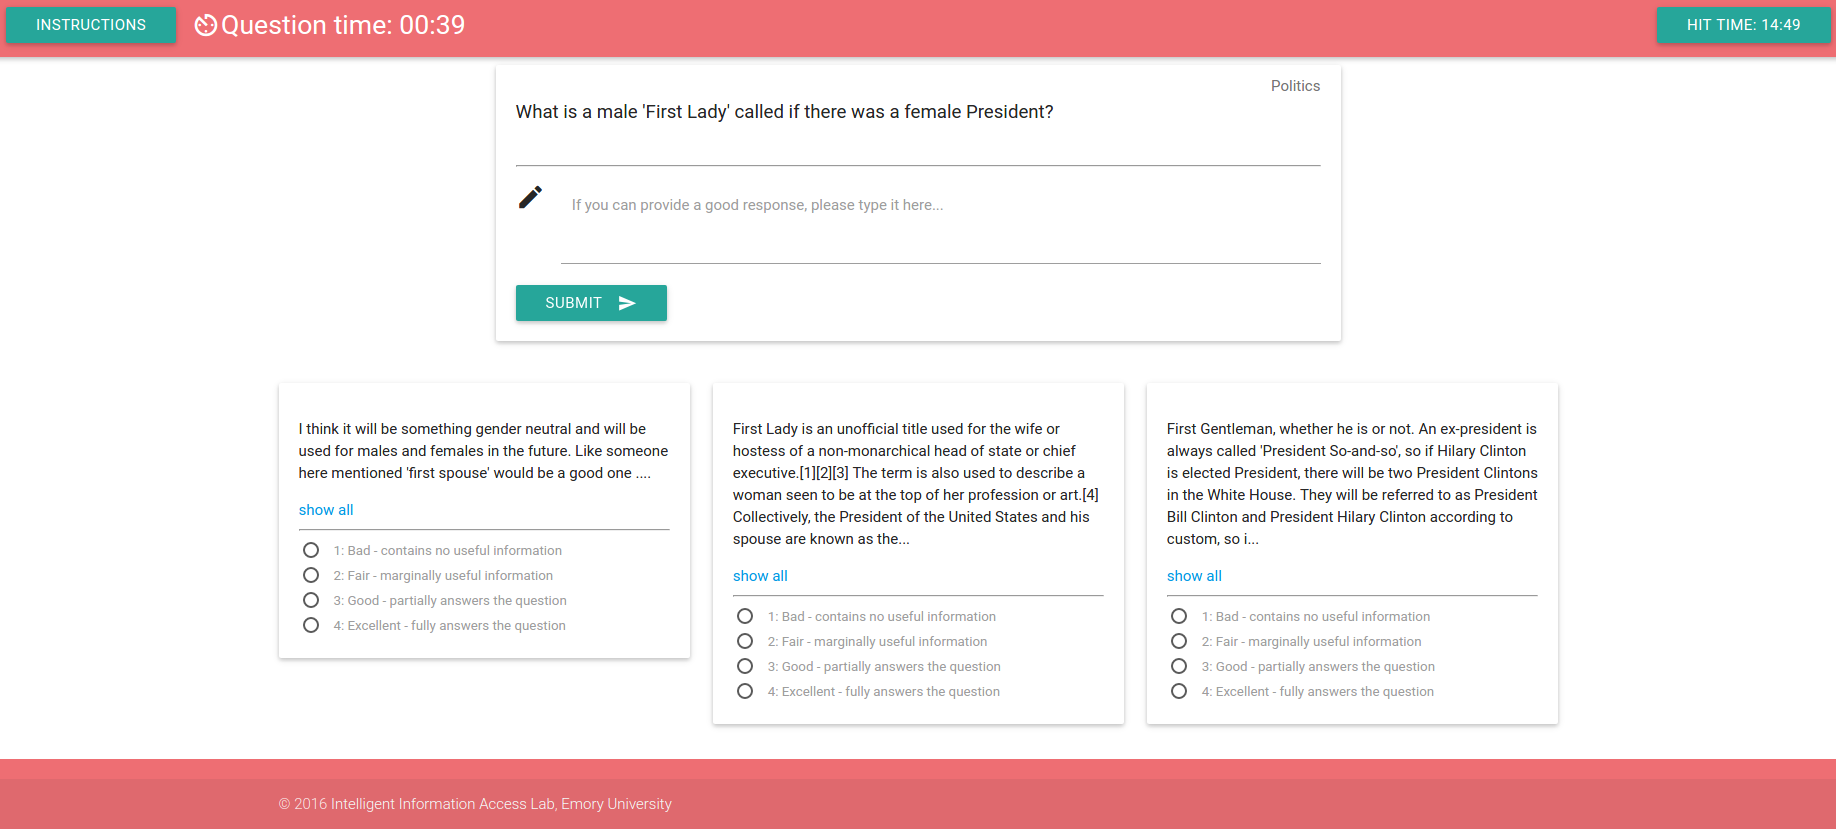
\includegraphics[width=\textwidth]{img/crowd_ui}
	\caption{User Interface for workers in our Crowd-Powered Question Answering system}
	\label{fig:crowd_ui}
\end{figure*}

The overall algorithm for obtaining crowd input for real-time question answering is the following:
\begin{enumerate}
\item When a system receives a question, it is posted to the workers, who will have 50 seconds to provide their input
\item Workers are asked to write an answer if they can provide one (it's optional)
\item Otherwise they are waiting for the answer candidates to arrive
\item When a system is done with generating and ranking candidates it posts top-7 scoring answers to the workers for the rating (which usually leaves $\sim$ 35 seconds for rating)
\item Workers receive a list of answers\footnote{Answers submitted by workers are also sent for ratings to all workers except the author} and rate them until the timer runs off. Each answer is rated on a scale from 1 to 4, using the official TREC LiveQA rating scale:
	\begin{itemize}[noitemsep,topsep=0pt]
    \item 1 -- Bad: contains no useful information
    \item 2 -- Fair: marginally useful information
    \item 3 -- Good: partially answers the question
    \item 4 -- Excellent: fully answers the question
    \end{itemize}
\item The interface displays 3 answers at a time, when an answer gets rated, it disappears and its place is taken by another answer from the pool. The interface displays only the first 300 characters of the answer, which was experimentally shown to be enough on average to make a good judgment.
Full answer can be revealed upon clicking the ``show all'' link.
\item When the timer runs off, the question and all the answers disappear, and workers wait for the next question
\end{enumerate}

To hire the workers we used Amazon Mechanical Turk platform\footnote{http://mturk.com}.
Since the challenge was to run the system ``live'' over the period of 24 hours, we adapted the retainer model to our question-answering task, inspired by its success in existing research~\cite{bernstein2011crowds,bigham2010vizwiz}.
Specifically, to obtain an even distribution of workers over the 24-hour period of the TREC LiveQA shared task, we posted 10 tasks every 15 minutes, and they expired after the next set of tasks became available.
Since not all assignments were accepted by some worker right away, the number of workers for each question varied and could be greater than 10.
When a worker first gets to our crowdsourcing interface, she is shown task instructions (Table \ref{table:crowd_instructions}) and asked to wait for the questions to arrive.
The workers were paid \$1.00 for the whole 15 minutes task, no matter how many questions they got\footnote{In TREC LiveQA task questions are sent to the systems one by one, therefore there is no concurrency, however the delays between the questions are possible}.

We should note, that the setup of TREC LiveQA shared task was very favorable for this model, as the questions were arriving almost every minute uniformly over 24 hour period, which minimizes the waiting time and worker idleness problem~\cite{Lasecki:2013:CCC:2501988.2502057}.
An interesting challenge, that we leave for future work, is how such a crowd-powered QA system can handle varying questions volume, while optimizing the costs.
~\cite{bernstein2012analytic} describes a number of techniques to optimize the costs of the retainer model.
It's also possible to reduce the latency associated with hiring new workers on a crowdsourcing platform, \textit{e.g.}, quikTurkIt approach of ~\cite{bigham2010vizwiz}.
Another idea, applied to question answering, is to prioritize the questions according to their predicted difficulty, \textit{i.e.}, we should allocate more workers to questions, for which the automatic system isn't confident in the generated answer, than to some easy questions.

\begin{table}[ht]
\centering
\begin{tabular}{| p{8cm} |}
\hline
\textbf{Instructions} \\
\hline
1. This HIT will last exactly 15 minutes\\
2. Your HIT will only be submitted after these 15 minutes\\
3. In this period of time you will receive some questions, that came from real users on the Internet\\
4. Each question has a time limit after which it will disappear and you will need to want for the next one\\
5. If you know the answer to the question, please type it in the corresponding box\\
6. At some point several candidate answers will appear at the bottom of the page\\
7. Please rate them on a scale from 1 (bad) to 4 (excellent)\\
8. Do not close the browser or reload the page as this will reset your assignment.\\
\hline
\end{tabular}
\caption{Crowdsourcing task instructions, displayed to the user when she first gets to the task}
\label{table:crowd_instructions}
\end{table}

\subsection{Answer re-ranking and selection}
\label{sec:system:reranking}

The last stage in CRQA is answer re-ranking, which aggregates all the information received from the crowdsourcing and produces the final answer to the question.
The input of the re-ranking module is a set of candidate answers with quality ratings provided by the crowd workers.
Candidates can include the answers posted by the workers, which might also be rated, if workers had enough time to do that.
We trained another learning to rank model\footnote{For convenience, we used Gradient Boosting Regression Trees~\cite{friedman2002stochastic} from scikit-learn Python package.} to re-rank the answers given all available crowdsourcing information.
The re-ranking model was trained on a subset of questions from TREC LiveQA 2016 run\footnote{We should note, that the experiments with trained re-ranking model was conducted after the LiveQA final run. For the shared task we used a simpler heuristic-based re-ranker, described in the next Section}.
To estimate the quality of answers, that were given to workers for rating, including worker-generated answers, we turned to the traditional batch-model crowdsourcing.
Workers were asked to label each answer on a scale from 1-bad to 4-excellent.
Then, a subset of the questions was used for training, while the rest was used to estimate the quality of the models.

The features, used for answer re-ranking are listed in Table \ref{table:reranking_features}.

\begin{table}[ht]
\centering
\begin{tabular}{| p{8cm} |}
\hline
\textbf{Answer-based} \\
\hline
--- The length of the answer \\
--- Source of the answer (Crowd, Web, Yahoo! Answers, Answers.com or WikiHow.com)\\
--- Original rank of the candidate answer or -1 for answers provided by the crowd workers\\
\hline
\textbf{Worker ratings} \\
\hline
--- Number of ratings provided\\
--- Minimum, maximum, median and average ratings\\
\hline
\end{tabular}
\caption{The list of features used for answer re-ranking based on crowdsourcing input}
\label{table:reranking_features}
\end{table}

CRQA sorts the candidates by the quality score predicted by the model, as returns the top candidate as the final answer.

